\begin{figure}[b]
    	\centering
    	\begin{minipage}{0.45\textwidth}
    		\centering
    		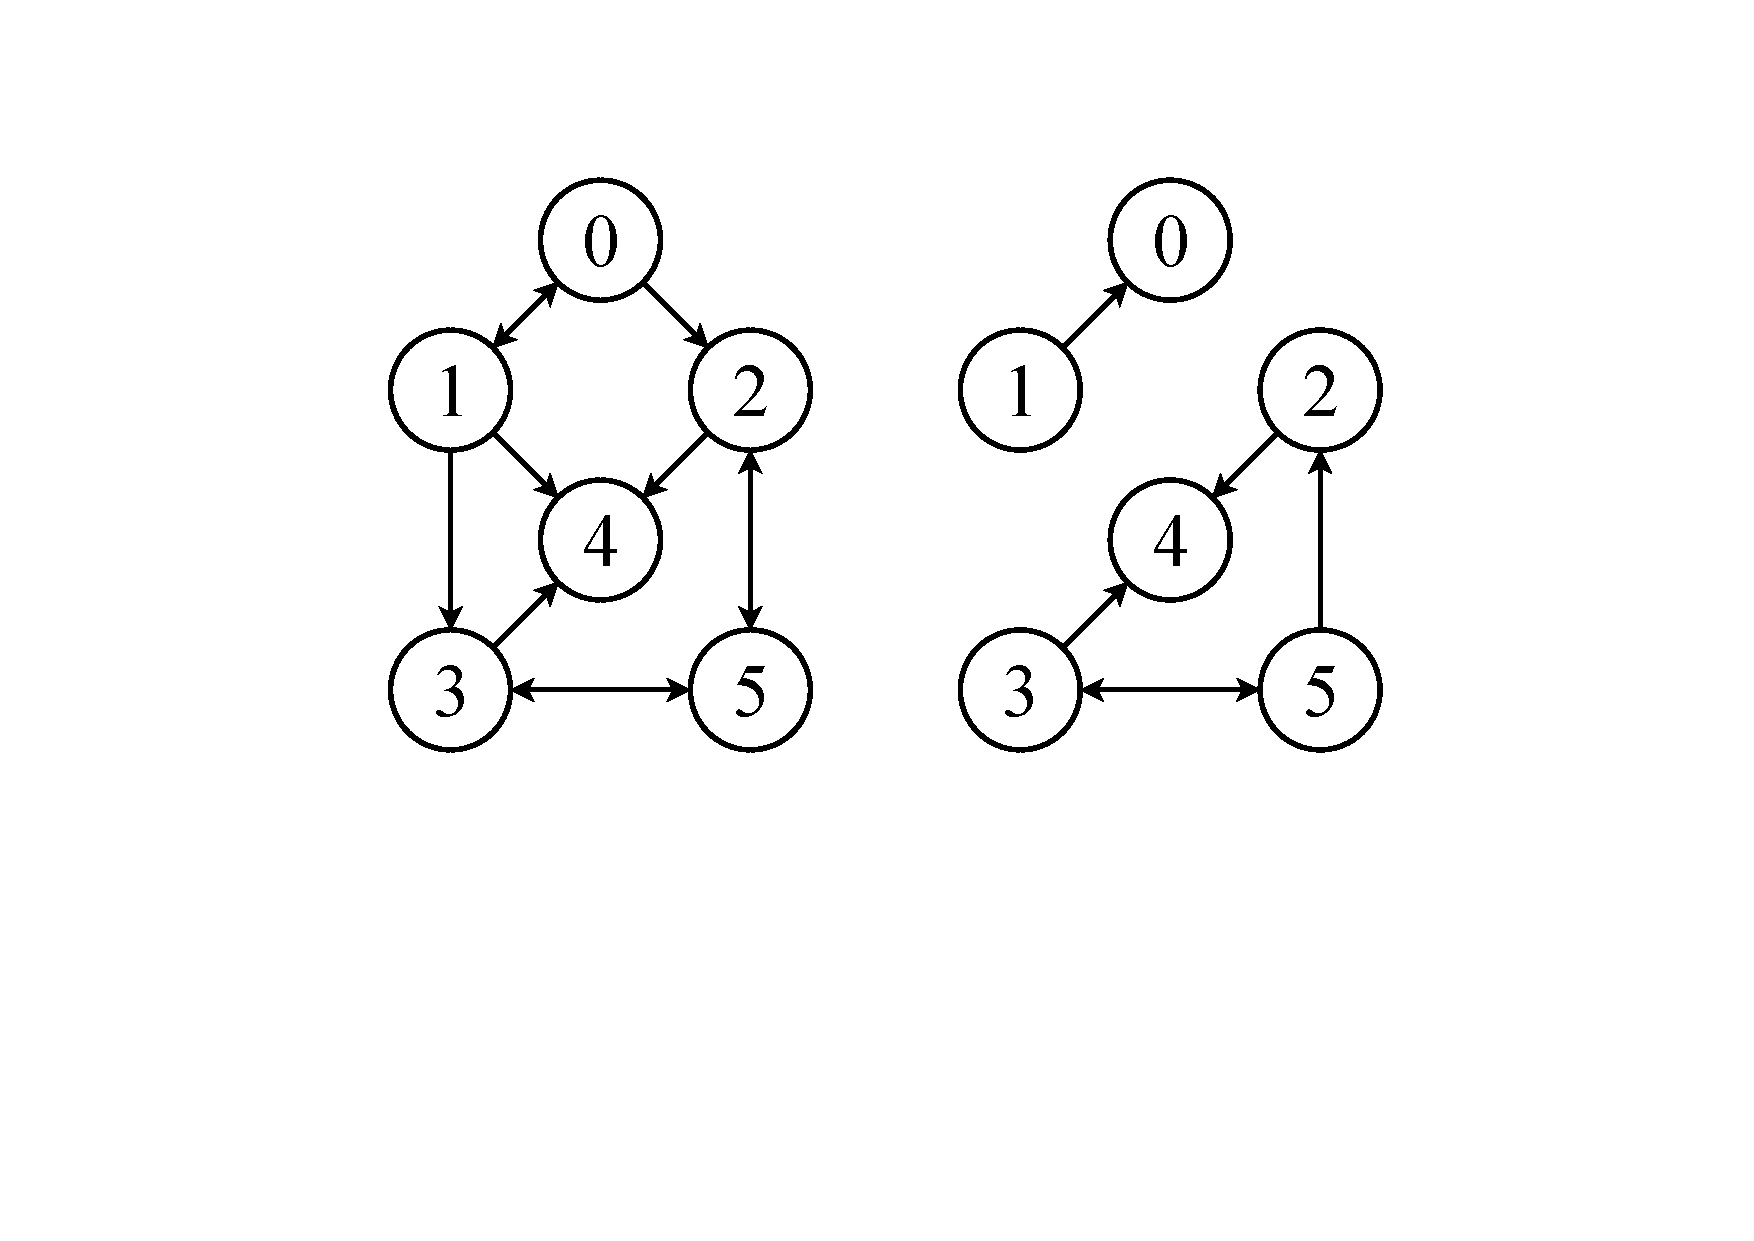
\includegraphics[scale=.35, clip, trim=180 230 440 80 ]{img/arte/graphs-BFS-F1.pdf}
    		
    		(a)
    	\end{minipage}
    	\begin{minipage}{0.45\textwidth}
    		\centering
    		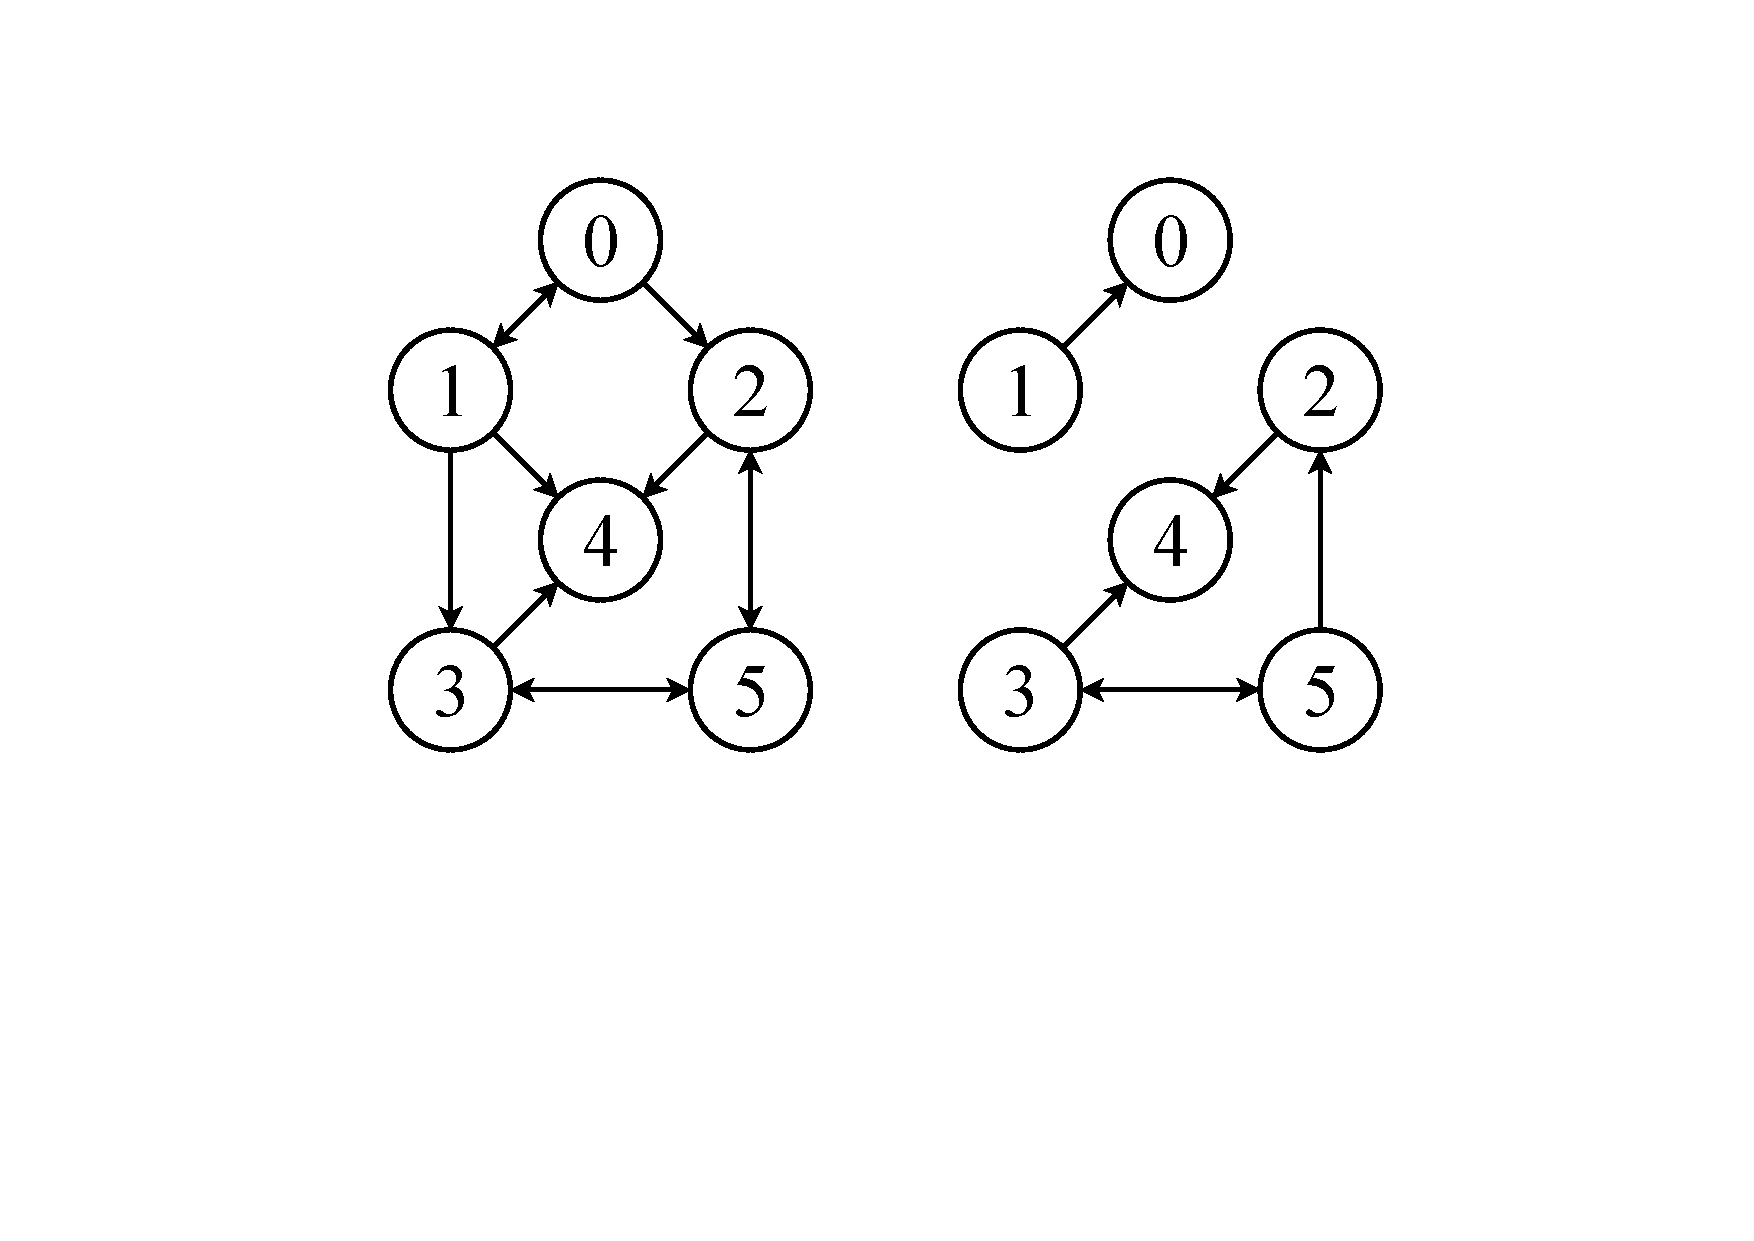
\includegraphics[scale=.35, clip, trim=450 230 170 80]{img/arte/graphs-BFS-F1.pdf}
    		
    		$T = \{2, 2, 1, 0, 0, 0\}$
    		
    		(b)
    	\end{minipage}

    \caption{Ejemplo de Fase 1 de BFS. (a) Índices asignados a los nodos. (b) Aristas restantes después de BFS, junto listado de recorrido $T$.}
    \label{fig:bfs1}
\end{figure}
